\chapter{基于反事实多智能体学习的图像场景图生成方法}

\section{问题描述}

本文
\begin{figure}[htbp]
    \centering
    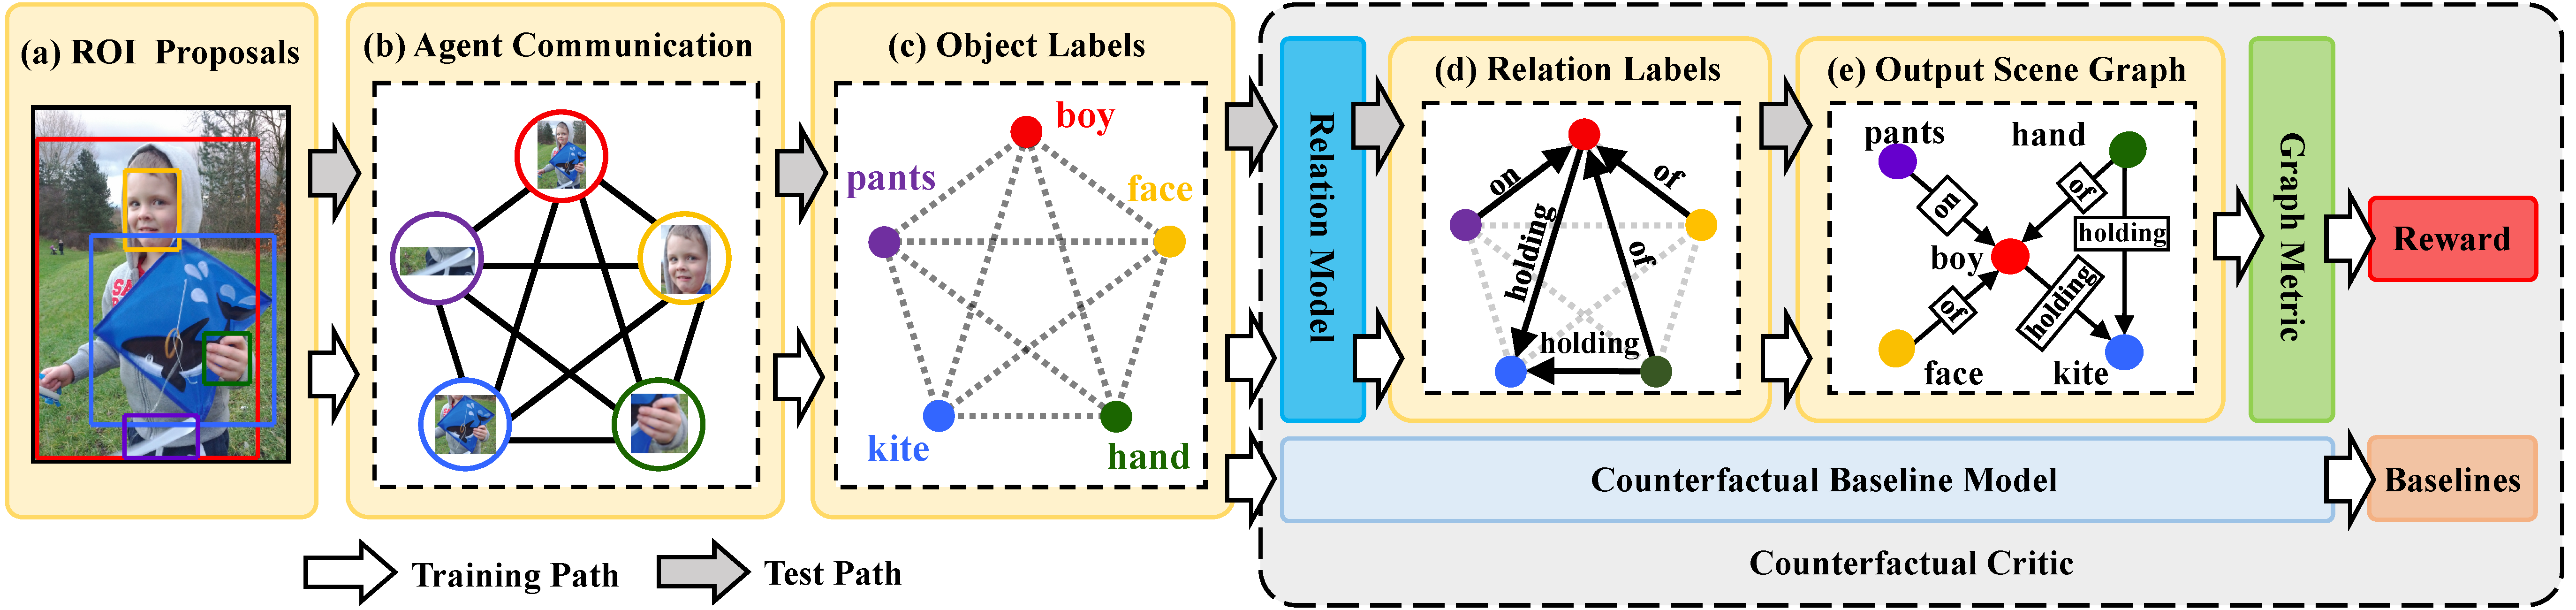
\includegraphics[width=\linewidth]{chapter4/res/architecture.pdf}
    \caption{motivation}
    \label{xx}
\end{figure}

\begin{figure}[htbp]
    \centering
    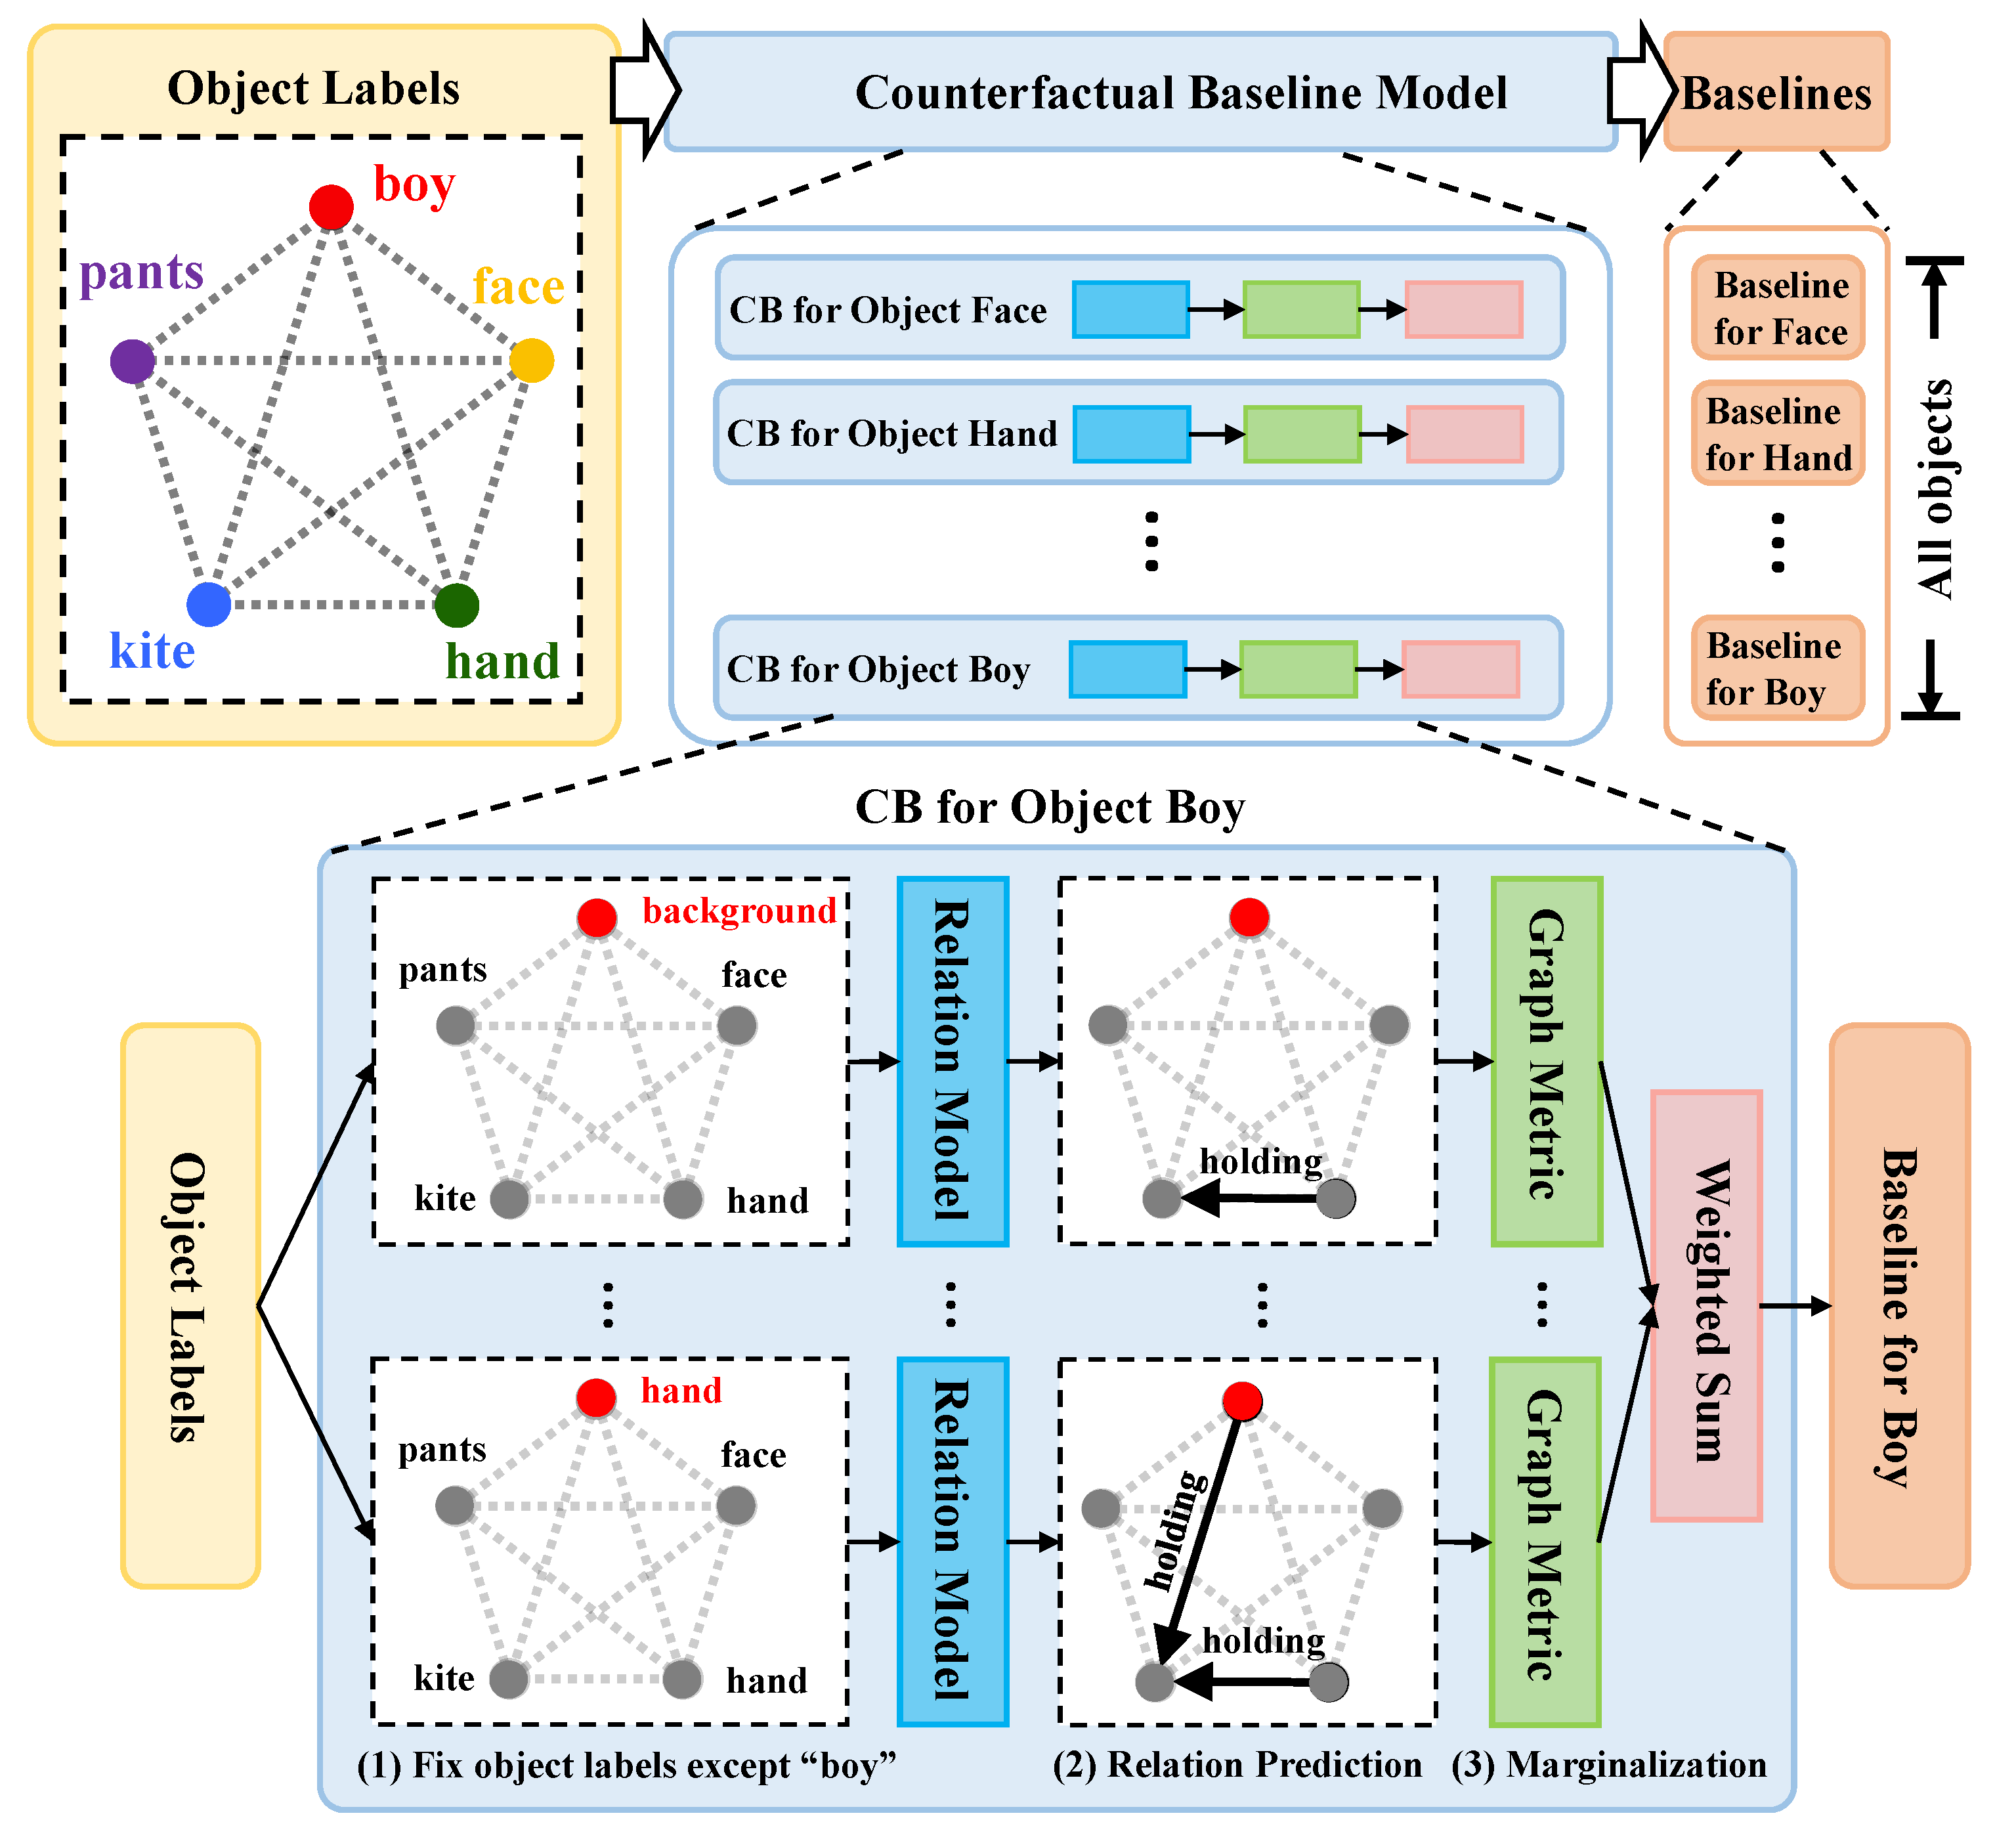
\includegraphics[width=\linewidth]{chapter4/res/baseline.pdf}
    \caption{motivation}
    \label{xx}
\end{figure}

\begin{figure}[htbp]
    \centering
    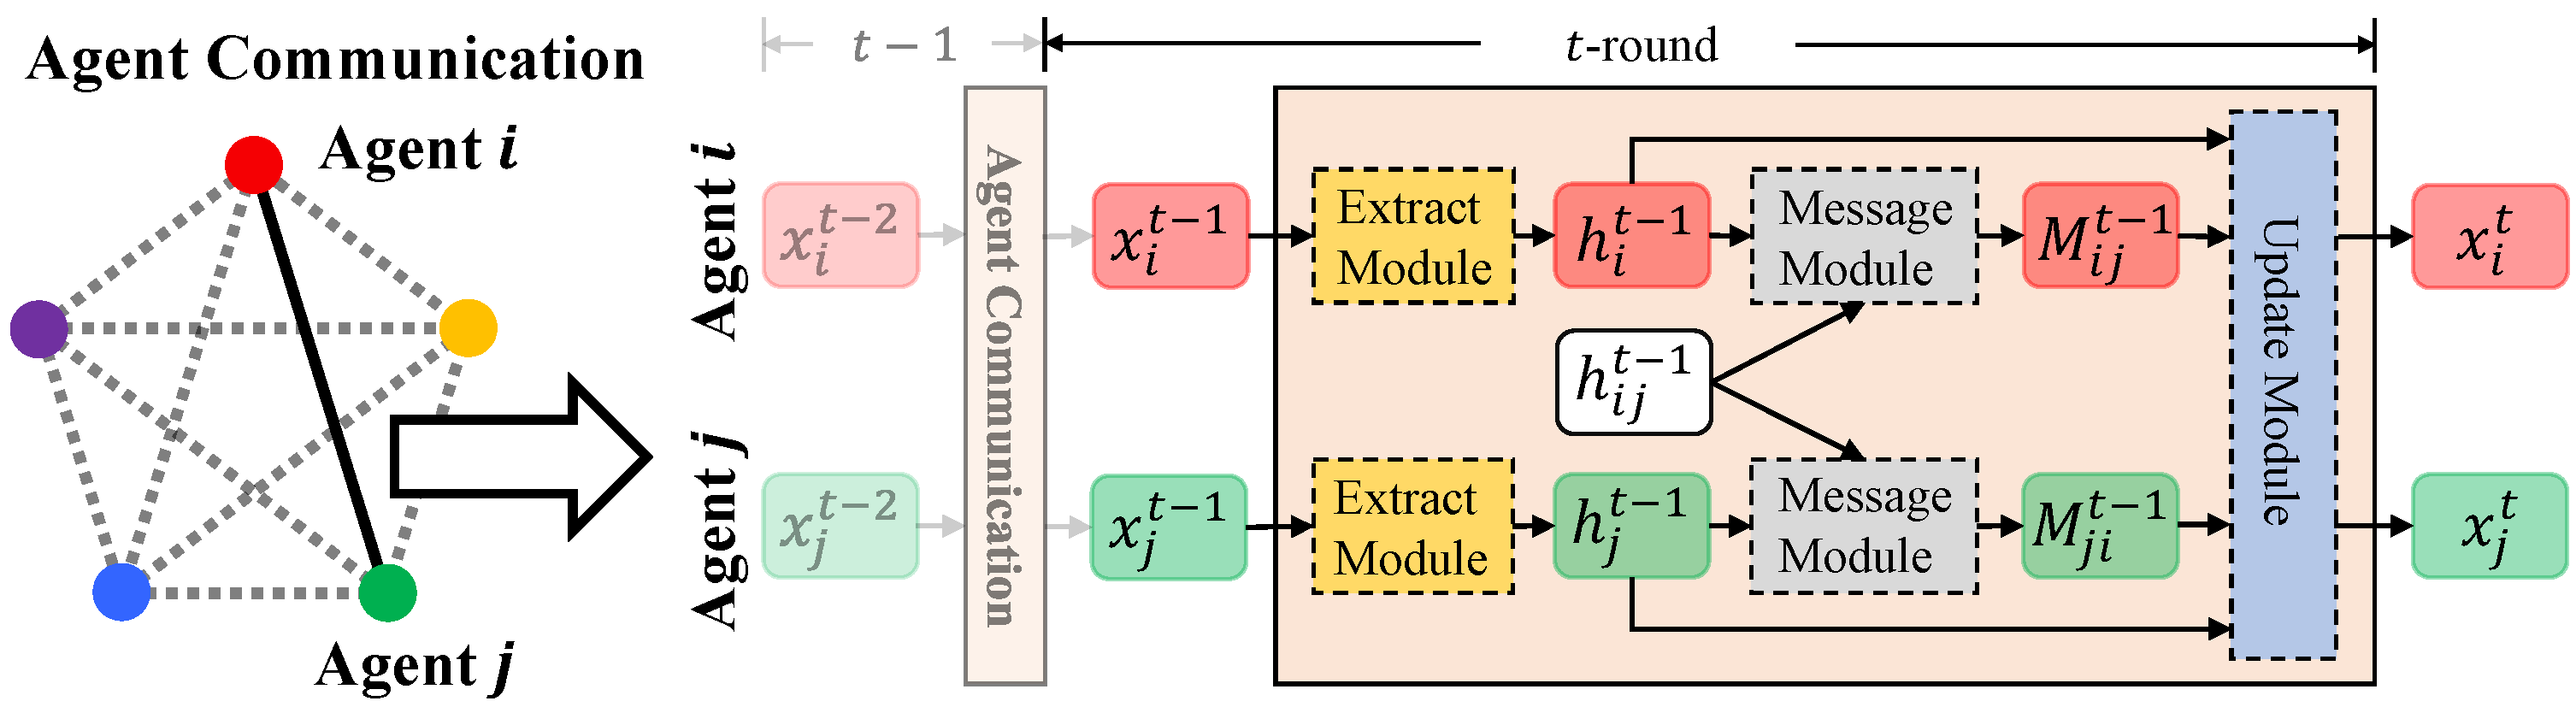
\includegraphics[width=\linewidth]{chapter4/res/communication.pdf}
    \caption{motivation}
    \label{xx}
\end{figure}

\begin{figure}[htbp]
    \centering
    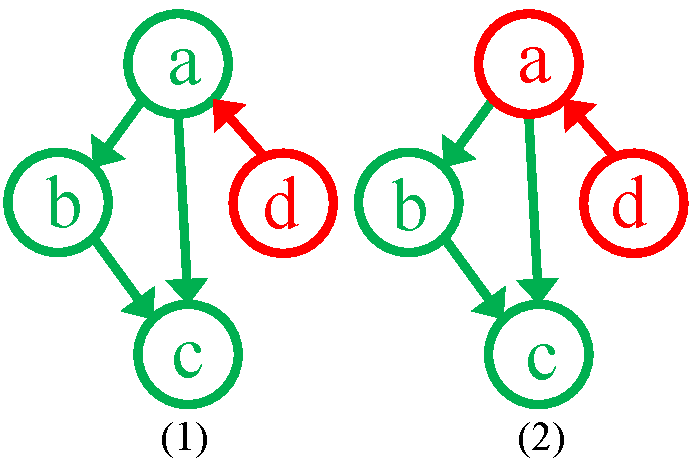
\includegraphics[width=\linewidth]{chapter4/res/local_sensitive.pdf}
    \caption{motivation}
    \label{xx}
\end{figure}

\begin{figure}[htbp]
    \centering
    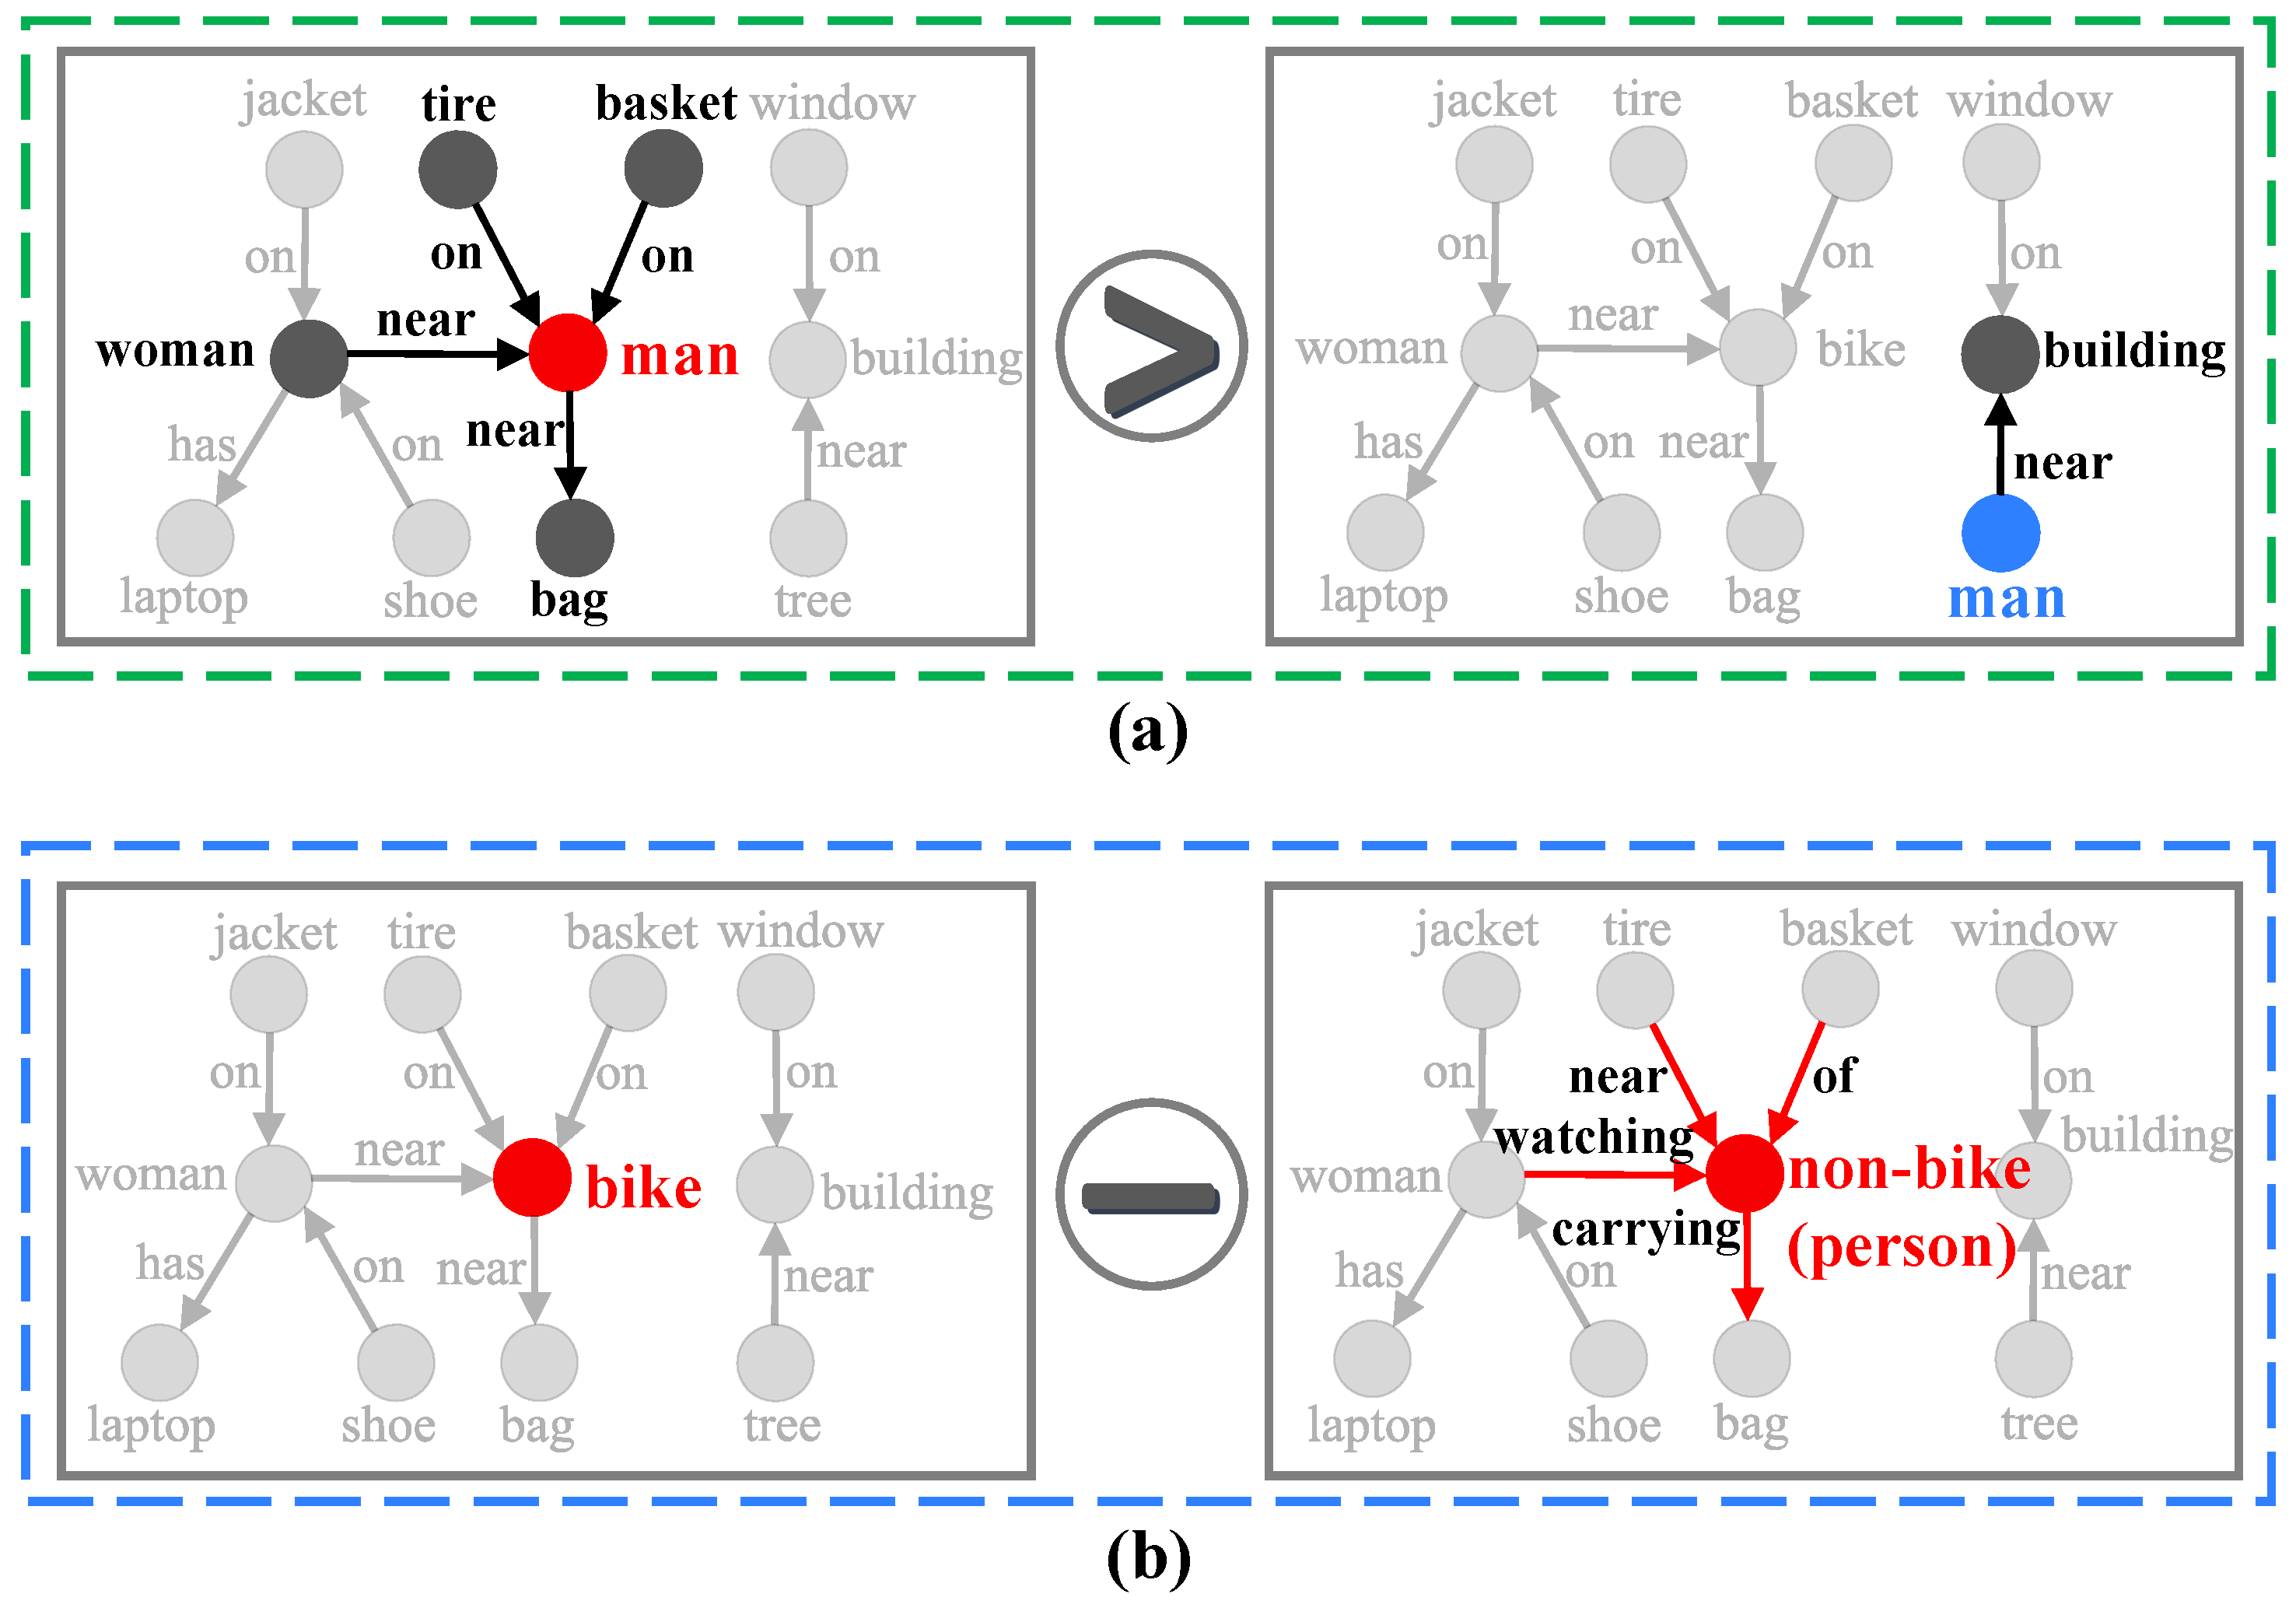
\includegraphics[width=\linewidth]{chapter4/res/motivation.pdf}
    \caption{motivation}
    \label{xx}
\end{figure}

\begin{figure}[htbp]
    \centering
    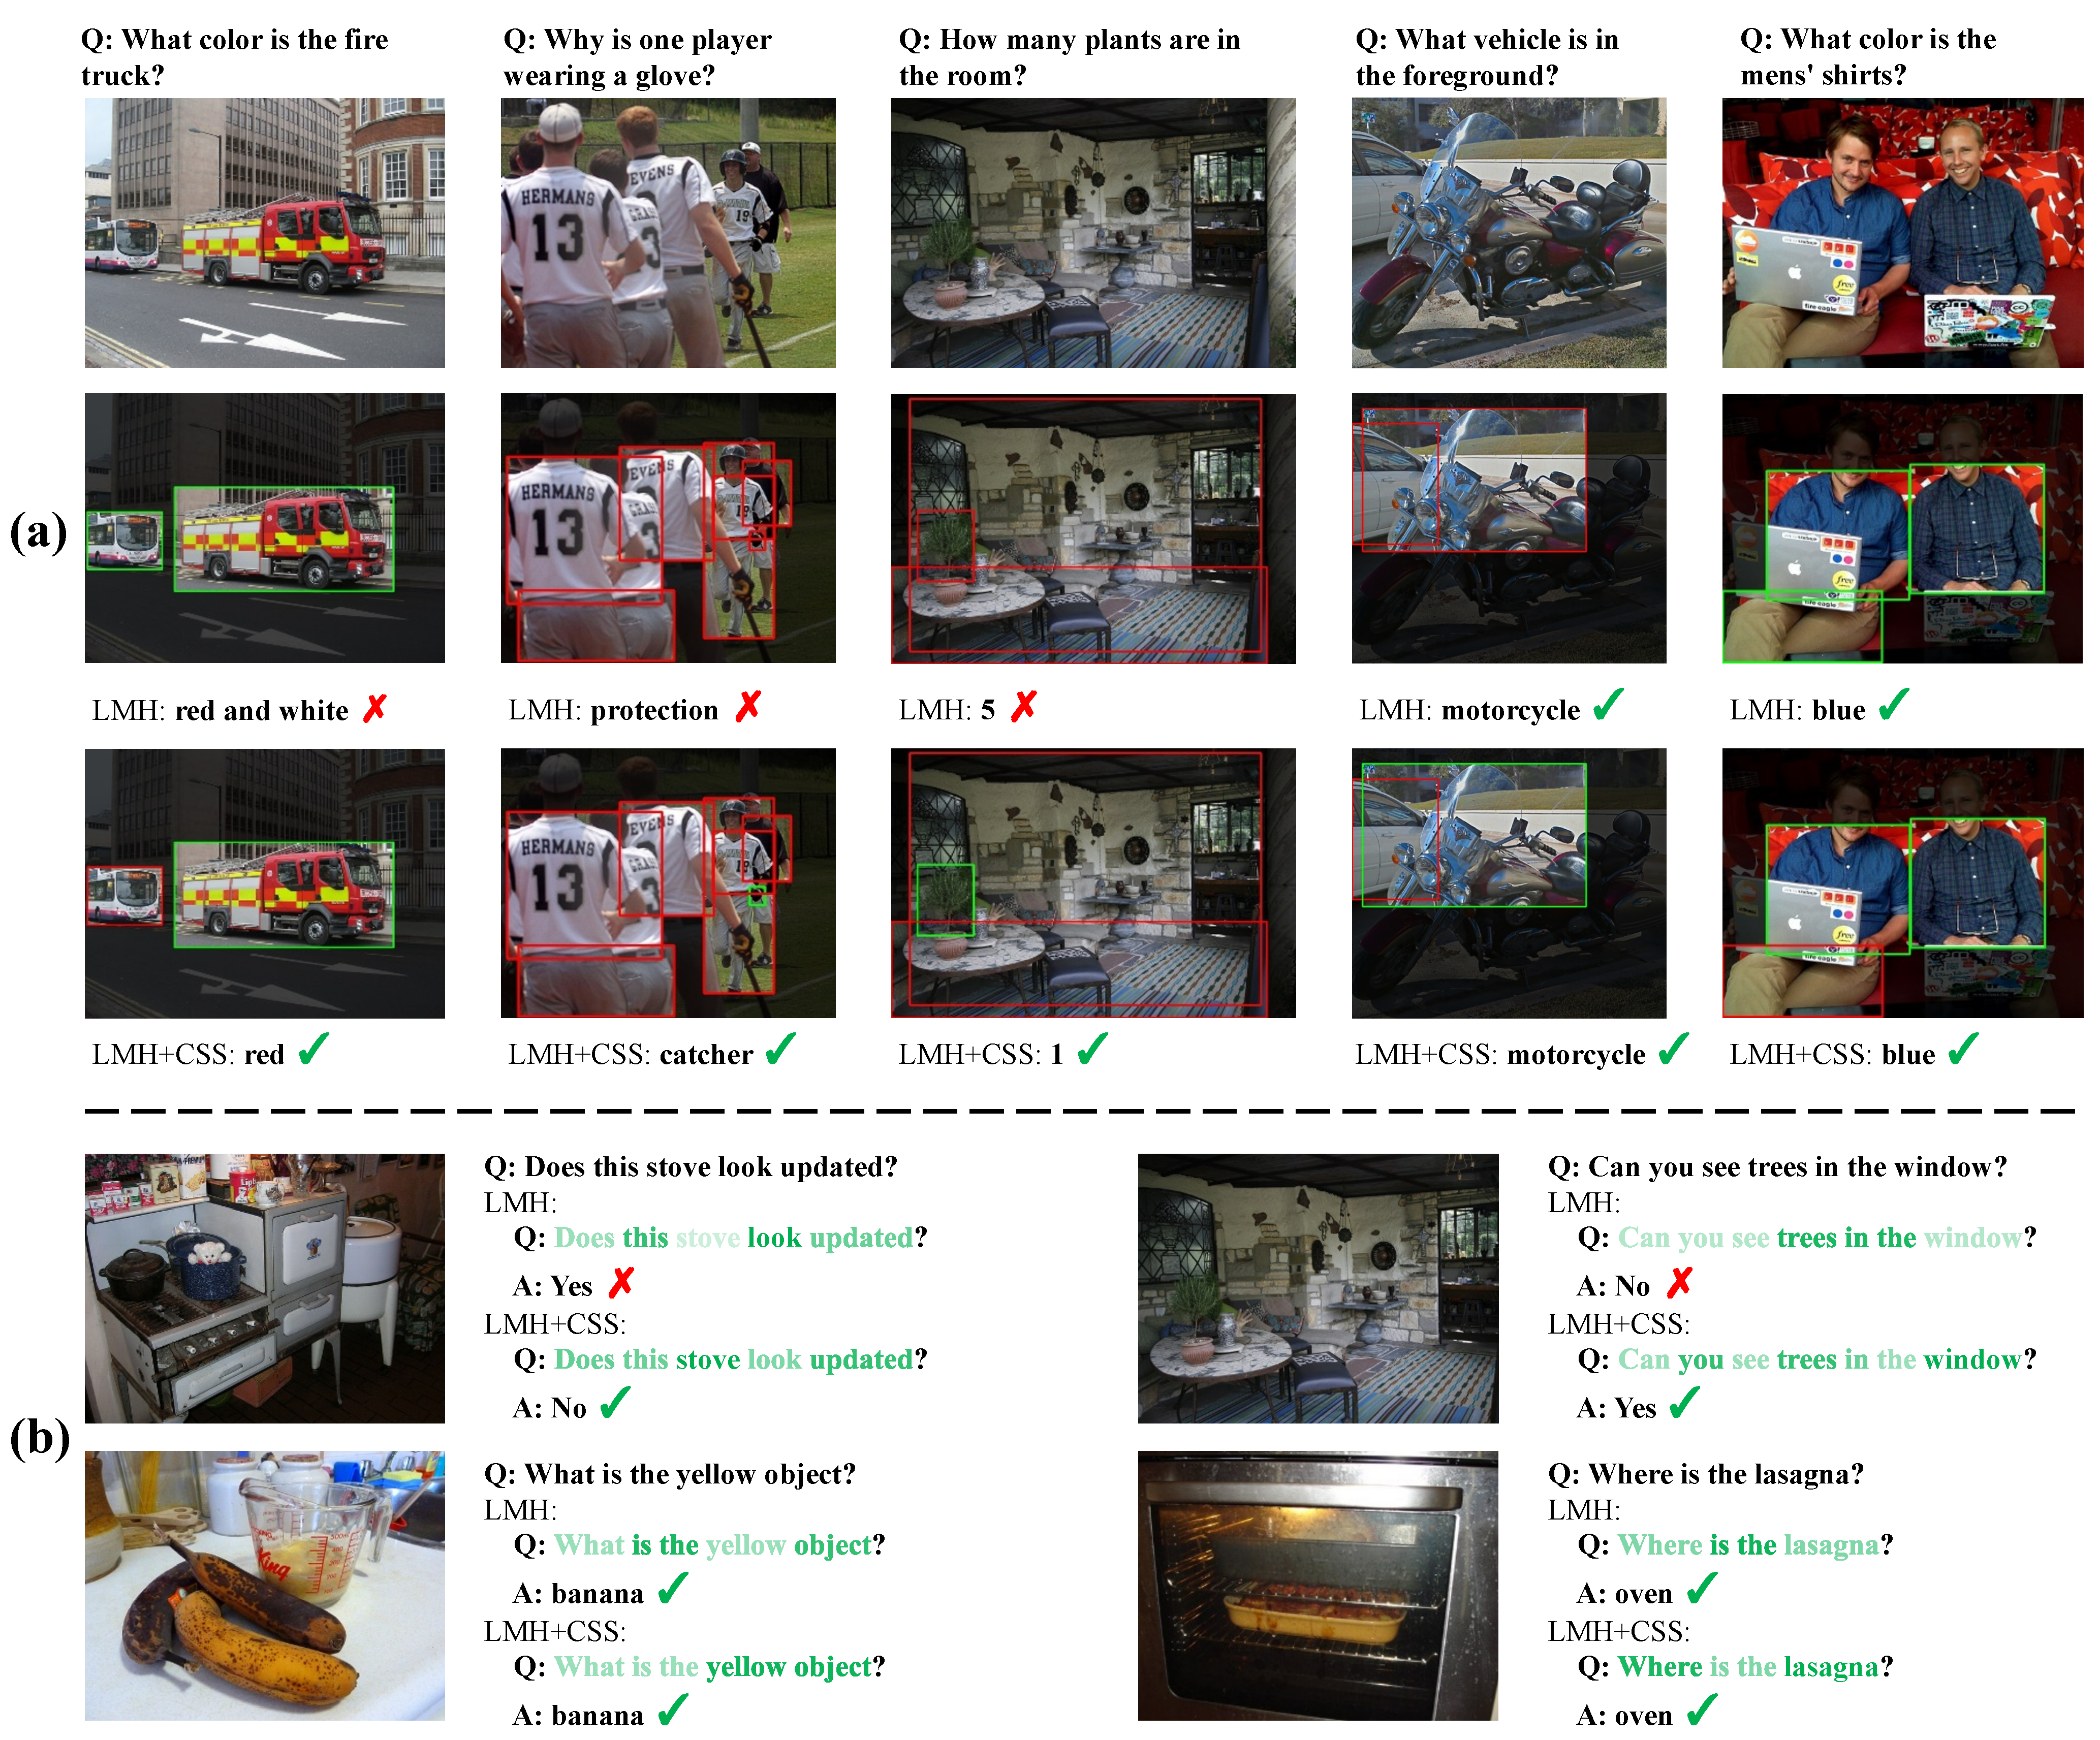
\includegraphics[width=\linewidth]{chapter4/res/visualization.pdf}
    \caption{motivation}
    \label{xx}
\end{figure}



\section{反事实多智能体学习}

\section{实验设置与性能对比}
\subsection{图像场景图生成数据集与实验设定}

\noindent{\kaishu{图像场景图生成数据集}}:我们使用目前最大的场景图数据集Visual Genome(VG) ~\cite{krishna2017visual}。为了与现有工作能够公平地进行比较,我们采用与现有工作相同的数据集划分和预处理~\cite{xu2017scene, zellers2018neural, newell2017pixels, yang2018graph, herzig2018mapping}。处理后的图像数据共包含150个物体类别和50个视觉关系类别。每张图像平均有11.5个物体和6.2个视觉关系。整个数据集中,70\%的图像数据当成训练集,30\%的图像数据当成测试集。


\noindent{\kaishu{实验设定}}:参考现有的文献~\cite{xu2017scene, zellers2018neural, jae2018tensorize},我们在三种实验设定下评估场景图生成质量:
\begin{asparaenum}
\item 视觉关系分类(PredCls):给定图像、所有的物体框和物体类别,模型需要预测所有的物体组合的视觉关系;

\item 场景图分类(SGCls):给定图像和所有的物体框,模型需要预测所有物体类别以及所有物体组合的视觉关系;

\item 场景图生成(SGDet):给定图像,模型需要检测物体框、预测所有物体类别以及所有物体组合的视觉关系。
\end{asparaenum}

对于视觉关系中物体框检测来说,需要主语(subject)和宾语(object)与真实准确物体框的交并比(IoU)均大于0.5。按照惯例,我们使用Recall@20(R@20)、Recall(R@50)和Recall(R@100)作为场景图生成质量的评价指标。


\subsection{实验细节}


\noindent{\kaishu{物体检测器}}:为了公平地与现有工作进行对比,我们采用了与~\cite{zellers2018neural}相同的物体检测器。具体来说,它是以VGG网络~\cite{simonyan2015very}为主干网络,然后锚框的大小和长宽比与YOLO-9000~\cite{redmon2017yolo9000}设置一样, 然后用RoIAlign~\cite{he2017mask}代替RoIPooling。


\noindent{\kaishu{训练细节}}:我们参照之前的策略梯度的工作,将整个训练过程分成两个阶段,并且先使用监督训练对模型进行参数初始化。在监督训练过程中,我们将RoIAlign层之前的参数都固定住,


\noindent{\kaishu{速度与正确率的权衡}}:在策略梯度的训练过程中,完整的反事实评论家的计算需要对所有可能的物体类别进行加权,通常需要非常多的时间(如:对于64个智能体,每个智能体共有151种物体类别选择,则需要超过9600次($\approx 151 \times 64$)的评估计算)。幸运的是,我们注意到只有极少数的类别有较大的预测概率。为了速度与正确率之间的权衡,我们只对背景(background)和预测概率最高的两种类别进行求和来对所有的类别进行近似。在我们的实验中,这样的实验设定可以把速度提升70倍,同时维持相同的实验效果。


\noindent{\kaishu{SGDet的后处理}}: 对于场景图生成任务(SGDet),为了与之前的工作~\cite{zellers2018neural,zhang2019graphical}公平地进行对比,我们采用相同的后处理操作。具体来说,在对每个RoI预测出物体所有类别的概率分布之后,我们对每个类别使用一次非极大值抑制来确定最终的物体类别,以及对应类别的位移偏置。在我们的实验中,非极大值抑制的IoU阈值设置为0.5。

\section{本章小结}